\chapter{Experiment Setup}
\label{chap:design}
In Chapter \ref{chap:threat_model}, we discussed the threat modelling and risk analysis of an OpenID Connect application implemented using PKCE on a cloud environment. The threat modelling provided an in-depth understanding of potential attack vectors and risks that could compromise the cloud-based application using the OpenID Connect Protocol. Building upon the insights gathered from the threat modelling exercise (See \ref{subsec:stride}), this chapter will focus on designing a prototype to address some identified threats. In particular, the very high and high threats will be mitigated. See Table \ref{table:risk_assessment}. 

This chapter will outline the implementation decisions and design choices undertaken to address identified risks. The objective is to establish a secure, scalable, and efficient cloud-based authentication system utilising Proof Key for Code Exchange (PKCE) on Amazon Web Services (AWS).

\section{Cloud Provider}
\label{sec:cloud_provider}
Designing and deploying a cloud-based application requires us to choose one of the many providers that offer such services as Microsoft Azure, Google Cloud Platform (GCP), and Amazon Web Services (AWS). Each of these popular platforms offers unique advantages and different service offerings. 

However, for this project, AWS is the preferred platform as it is the leader in the cloud services industry, with a vast global infrastructure that ensures reliability and scalability. \cite{aws_leader} states that it holds the most shares as a favoured vendor, with 31 per cent in the first quarter of 2024. Not only is AWS a widely adopted cloud platform, but it is also compliant with ISO 27001 and GDPR \citep{aws_iso}. In addition to the advantages of compliance, AWS offers extensive tools for prototyping and testing, namely Localstack.

\subsection{LocalStack for AWS Simulation}
LocalStack is a tool that allows developers to simulate AWS services locally, making it an excellent choice for rapid development and testing. With LocalStack, developers can build applications locally using AWS-like services such as Lambda, API Gateway, and more without needing to deploy code to the cloud \citep{localstack}. By mimicking the AWS environment, LocalStack allows developers to work on cloud-native applications locally, reducing development costs and the need to register for an AWS account, which is cost-intensive. Such a simulation tool does not yet exist for Azure and GCP, creating a solid argument for using AWS.


\subsection{Limitations}
\begin{itemize}
    \item \textbf{Partial Service Emulation}: 
    LocalStack does not fully emulate all AWS services or features. Specific service behaviours might not be available or behave differently than in the AWS environment.
    
    \item \textbf{Performance Differences}: 
    Since LocalStack runs locally, its performance might not accurately reflect the AWS cloud's.
    
    
    \item \textbf{Version Mismatches}: 
    LocalStack may not continuously be updated in sync with AWS's latest services and API changes, potentially causing discrepancies between local development and production deployments.
    
    \item \textbf{Complex Setup}: 
    As application architectures grow more complex, configuring and maintaining a Local Stack with multiple services can become challenging and time-consuming. In addition, to run a local stack, one must understand and learn how to spin up an environment with required services. For example, one must also understand the principles of running and managing docker containers.
    
    \item \textbf{Limited Real-World Testing}: 
    While LocalStack is excellent for early development and testing, certain edge cases or AWS-specific behaviours may only be encountered in the natural cloud environment, necessitating additional testing after deployment.
    
\end{itemize}

\section{Architecture}
\label{sec:architecture}
After deciding to use AWS as the cloud provider in Section \ref{sec:cloud_provider}, the application's design is centred around AWS services such as API Gateway, Lambda Servers, and DynamoDB for the database. In this section, we will delve into the chosen services in detail. The deployment of the PKCE (Proof Key for Code Exchange) application for two tenants necessitates a database to store user data. For this project, we have evaluated two different approaches for a multi-tenant setup: one involving a single database with data isolation and another involving multiple databases per tenant. 

Figure \ref{fig:deployment_diagram_single} illustrates a deployment architecture in which a single database accommodates multiple tenants, storing all associated tenant and user-related data within this centralized system. Conversely, Figure \ref{fig:deployment_diagram_dual} illustrates the utilisation of databases for each tenant, whereby user data is stored in individual tenant databases, and a catalogue database maintains the records of these tenant databases. In this multi-database configuration, user data is segregated by the tenant, while the catalogue database facilitates the organisation of tenant data, thereby ensuring a clear separation of data.



In \cite{niemela2023implementing}, the advantages and disadvantages of single and multiple databases per tenant are discussed. It argues that the multi-tenant application with multiple databases balances performance and security. This approach allows the databases to scale according to the needs of each tenant. It provides the capability to implement granular security measures such as encrypting specific data, maintaining access controls, and generating clear access logs. These features reinforce the data model's Confidentiality, Integrity, and Availability (CIA) principle. However, this approach also has drawbacks compared to its single database counterpart. Managing multiple databases introduces overhead and increases the likelihood of misconfiguration, as each database operates independently. Despite the additional configuration and maintenance complexity, the approach with multiple databases is a viable solution for the application. The security benefits of using the multi-databases are as follows:

\begin{itemize}
    \item \textbf{Isolation of Sensitive Data}: Unlike a single database for a multi-tenant application, the data are isolated from each other entirely. Should a security vulnerability be discovered, the damage will be limited to one data set rather than exposing all sensitive information. 
    
    \item \textbf{Improved performance}: Separation of tenant data allows a more efficient way of accessing the data. Using one table in the database does not affect the other. Furthermore, the database can be configured according to each tenant's needs to scale it up and down, increasing performance. This, in terms of simplifying the queries to retrieve data, also reduces possible SQL attacks due to more straightforward queries.
    
    \item \textbf{Custom Encryption Keys}: Using two tables, separate encryption keys for each table, enhancing the data security and ensuring that each data set has independent encryption controls that can be configured. Should one encryption key be compromised, the other remains secure. 
 
\end{itemize}

\begin{figure}[h!]
\label{fig:deployment_diagram_single}
\centering
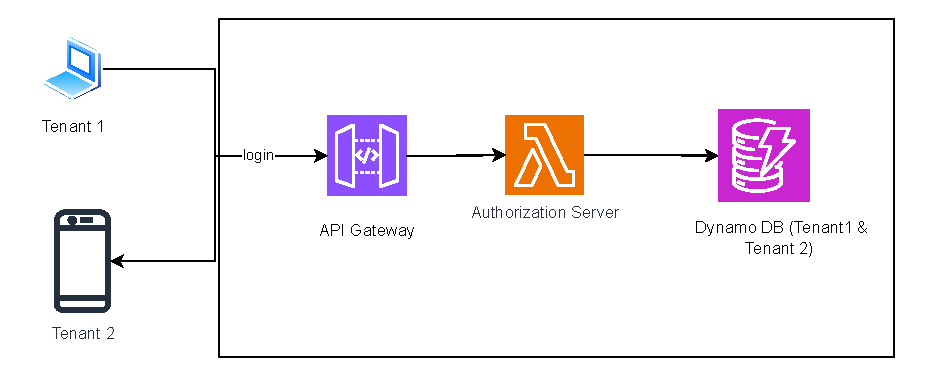
\includegraphics[width=\textwidth]{pics/deployment_diagram_single.pdf}
\caption{Deployment diagram with Single Database}
\end{figure}

\begin{figure}[h!]
\centering
\label{fig:deployment_diagram_dual}
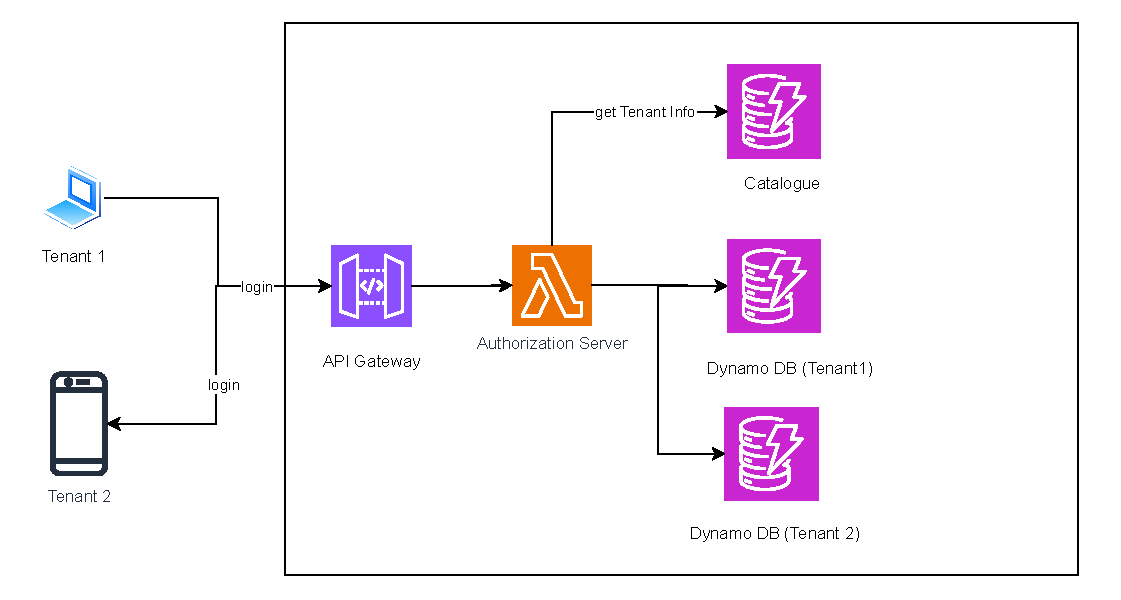
\includegraphics[width=\textwidth]{pics/deployment_diagram_multi.pdf}
\caption{Deployment diagram with Multi Database}
\end{figure}


\subsection{Overview of the Deployment Architecture}
This section discusses the AWS services used to implement the PKCE flow for two tenants with multiple databases (See Figure \ref{fig:deployment_diagram_dual}). The deployment architecture consists of the following main components:

    \paragraph{API Gateway}: This is the public interface for the application that provides endpoints for the clients to perform login and authorisation. This service is responsible for routing the requests to the appropriate Lambda based on the path. The API gateway can also be configured to restrict access using the API key and limit the request using throttling, preventing unwanted access and reducing Denial of Service attacks.
    
    \paragraph{Lambda Functions}: Lambda functions are serverless functions that contain the logic that handles the PKCE OpenID Connect. It is responsible for storing and retrieving the PKCE code verifiers, processing the callback, authenticating and authorising users, and generating access and refresh tokens. In contrast to regular servers, Lambdas are more lightweight, spun up only when needed, and terminated after their runtime. In addition, AWS Lambdas uses a specialised virtual machine manager (VMM) called Firecracker, which helps with container isolation, as AWS uses shared hardware protecting from microarchitectural attacks \citep{lambda_vm_firecracker}. Advantages such as resource optimization and the lack of container orchestration and setup for the prototype make it a proper candidate.
    
    \paragraph{DynamoDB Databases}: DynamoDB is a AWS proprietary NOSQL database. This database is used as it is easy to use and can be easily integrated with the other services that would speed up the implementation of the prototype. These databases will store user-specific data, such as user information and credentials, and code verifiers associated with each user session. The database is configured per tenant so that each tenant will have a database. By storing PKCE code verifiers and tenant data in separate tables, we can isolate sensitive information based on its purpose. If one table’s access were compromised, the other table’s data would remain secure. This is particularly useful when dealing with data regulated under compliance frameworks like GDPR or HIPAA, as it helps limit data exposure. DynamoDB, also like AWS lambda, abstracts away all server management and provisioning tasks \citep{dynamodb}. Therefore, using Dynamodb allows more flexibility and complex SQL queries are not required for data structure as they can be stored in a flexible schema design and fit the project.\newline

Deploying an application using AWS API Gateway, AWS Lambda, and multiple DynamoDB tables offers a highly secure and scalable architecture that aligns with modern best practices for serverless computing and data protection. A key advantage of using two distinct DynamoDB tables is the ability to isolate different types of data based on their sensitivity or usage patterns. For instance, sensitive data such as personally identifiable information (PII) can be stored in one table, while less critical operational data resides in another. This separation enhances security by reducing the risk of unauthorised access or exposure; if a breach occurs, the impact is contained to only one table, making it easier to manage and mitigate damage. Additionally, this setup allows for applying granular IAM (Identity and Access Management) policies, enabling fine-tuned control over who or what can access each table. This granular approach enforces the principle of least privilege, ensuring that users and services only have the permissions they need, ultimately minimising the risk of accidental or malicious access to sensitive data. The ability to tailor permissions at the table level makes it far easier to implement strict security measures, which is especially important for organisations handling sensitive information or subject to stringent regulatory requirements.

\section{Implementation}
This Section extends the design presented in Chapter \ref{chap:design}, focusing on implementing the Proof Key for Code Exchange (PKCE) authorisation flow for a dual-tenant environment. Using the multi-database architecture proposed in the design (refer to Figure \ref{fig:deployment_diagram_dual}), this implementation builds a foundational prototype of the OAuth 2.0 Authorisation Code flow with PKCE, adapted for a multi-tenant, serverless infrastructure. By leveraging modern, cloud-native technologies—including Node.js, TypeScript, and LocalStack—this prototype demonstrates a secure, efficient, and scalable user authorisation approach in a serverless multi-tenant application. The implementation focuses on the two critical endpoints: the authorisation endpoint \textbf{/authorize} and the token endpoint \textbf{/token} deployed in a cloud infrastructure, which forms the cornerstone of the OAuth 2.0 PKCE flow. The following sections discuss the implementation details and the tests conducted for the project.


\subsection{Technical Stack}
The technical stack forms the foundations of any software development project, comprising a carefully selected combination of programming languages, frameworks, libraries, and tools that enable the creation of robust applications. During the prototyping phase, selecting an appropriate technical stack is crucial, as it significantly influences development velocity, code quality, and the project's overall success. Moreover, security considerations are vital in stack selection, as well-established technologies often incorporate proven security practices and help mitigate potential vulnerabilities. To address these requirements and ensure a solid foundation for the prototype, the implementation leverages the following technology stack:

\begin{itemize}
    \item \textbf{Runtime Environment:} Node.js 18.x
    \item \textbf{Programming Language:} Javascript with TypeScript 5.6
    \item \textbf{Cloud Infrastructure:} AWS (simulated locally using LocalStack)
    \item \textbf{Database:} Amazon DynamoDB
    \item \textbf{Framework:} Serverless Framework
    \item \textbf{Infrastructure as Code:} Terraform and Terraform Local for localstack

\end{itemize}

\subsection{Development Dependencies}
A carefully selected set of dependencies was chosen to develop the prototype, enhancing the project's security, maintainability, testing, operability, logging, and performance. Each dependency was selected for a specific purpose, ensuring the system remains robust, efficient, and scalable throughout the development lifecycle. Table \ref{table:dev_dependencies} lists the dependencies used with its description, and table \ref{table:lint_testing_dependencies} lists the testing and linting dependencies. 

\begin{longtable}{|l|l|p{8cm}|}
\caption{Development Dependencies}
\label{table:dev_dependencies}
\hline
\rowcolor{grey!15}
\textbf{Dependency} & \textbf{Version} & \textbf{Description} \\ \hline
\endfirsthead
\hline
\rowcolor{grey!15}
\textbf{Dependency} & \textbf{Version} & \textbf{Description} \\ \hline
\endhead
\endfoot
\hline
\endlastfoot
argon2 & \textasciicircum 0.41.1 & A password hashing library implementing the Argon2 algorithm, designed for secure password storage. \\ \hline
axios & \textasciicircum 1.7.7 & A client for making HTTP requests in Node.js and browsers. \\ \hline
esbuild & \textasciicircum 0.24.0 & A fast JavaScript and TypeScript bundler and minified optimized for development and production builds.\\ \hline
hash-wasm & \textasciicircum 4.11.0 & A fast cryptographic hashing library using WebAssembly for efficiency. \\ \hline
jsonwebtoken & \textasciicircum 9.0.2 & A library to sign, verify, and decode JSON Web Tokens (JWT), commonly used for authentication and authorisation. \\ \hline
@types/aws-lambda & \textasciicircum 8.10.145 & TypeScript type definitions for AWS Lambda, providing type support for AWS Lambda functions. \\ \hline
@types/jsonwebtoken & \textasciicircum 9.0.7 & TypeScript type definitions for jsonwebtoken, helping with type safety when using JWTs in TypeScript code. \\ \hline
@types/node & \textasciicircum 22.7.7 & TypeScript type definitions for Node.js, providing type support for Node.js APIs in TypeScript projects.\\ \hline
typescript & \textasciicircum 5.6.3 & The TypeScript programming language, which adds static types to JavaScript to improve developer productivity and code quality.\\ \hline
uuidv4 & \textasciicircum 6.2.13 & A library to generate UUID (Universally Unique Identifier) version 4, primarily used for creating unique identifiers. \\ \hline
winston & \textasciicircum 3.15.0 & A flexible and popular logging library for Node.js, supporting multiple log transports. \\ \hline
winston-cloudwatch & \textasciicircum 6.3.0 & A transport for Winston allows logging to AWS CloudWatch for centralized logging and monitoring. \ \hline
zod & \textasciicircum 3.23.8 & A TypeScript-first schema validation library for parsing and validating inputs. \\ \hline
@aws-sdk/client-dynamodb & \textasciicircum 3.675.0 & AWS SDK Client for DynamoDB, used for interacting with Amazon DynamoDB from Node.js applications. \\ \hline
\end{longtable}


\begin{longtable}{|l|l|p{8cm}|}
\caption{Testing and Linting Dependencies}
\label{table:lint_testing_dependencies}
\hline
\rowcolor{grey!15}
\textbf{Dependency} & \textbf{Version} & \textbf{Description} \\
\endfirsthead
\hline
\rowcolor{grey!15}
\textbf{Dependency} & \textbf{Version} & \textbf{Description} \\
\endhead
\endfoot
\hline
\endlastfoot
fast-check & \textasciicircum 3.23.1 & A property-based testing library for generating random test cases and checking properties of your code. \\
\hline
jest-fuzz & \textasciicircum 0.1.2 & A fuzz testing library for Jest, used to test for unexpected edge cases. \\
\hline
@types/jest & \textasciicircum 29.5.14 & TypeScript definition for Jest enables type safety in Jest test cases. \\
\hline
@typescript-eslint/eslint-plugin & \textasciicircum 8.13.0 & ESLint plugin that provides TypeScript-specific linting rules. \\
\hline
aws-sdk-client-mock & \textasciicircum 4.1.0 & A mocking library for the AWS SDK, used in unit tests to mock AWS services like DynamoDB. \\
\hline
eslint & \textasciicircum 9.14.0 & A powerful linter for JavaScript and TypeScript that helps identify and fix coding issues. \\
\hline
eslint-plugin-security-node & \textasciicircum 1.1.4 & An ESLint plugin that identifies potential security vulnerabilities in Node.js code. \\
\hline
jstat & \textasciicircum 1.9.6 & A JavaScript statistics library that can be used for different statistical calculations, like mean, standard deviations, t-test, and chi-squared tests. \\
\hline
jest & \textasciicircum 29.7.0 & A JavaScript testing framework that supports unit tests, integration tests, and snapshot testing. \\
\hline
ts-jest & \textasciicircum 29.2.5 & A Jest transformer allows Jest to run TypeScript code directly. \\
\hline
typescript-eslint & \textasciicircum 8.13.0 & A set of tools that allow ESLint to analyse TypeScript code and enforce best practices. \\
\hline
\end{longtable}

\subsection{Infrastructure as Code}
Infrastructure as Code (IaC) is an approach to managing IT infrastructures, like infrastructure or services created by AWS, using configuration and machine-readable definition files \citep{iac}. This method replaces the manual process of creating infrastructure and allows automation to provision different components like databases, servers, and networking components. One of the main advantages of IaC is that it provides consistency in provisioning infrastructure as a code-like script, leading to more reliable deployments. In addition, IaC also helps in faster deployments, and as the infrastructure is written in code, static analysis tools to check vulnerabilities are possible.

IaC is widely used in the industry to practice DevOps and continuously deploy. Many tools, such as AWS CloudFormation, AWS Cloud Development Kit (CDK), Ansible, and Terraform, are available to manage complex infrastructure. For this project, Terraform was chosen due to its status as one of the most widely used IaC tools, backed by a robust community and reusable modules \citep{terraform}.

Additionally, an essential aspect of this project is integrating the IaC tool with LocalStack, a platform that simulates AWS services locally for testing purposes. Terraform's compatibility with LocalStack is well-documented through tflocal, which allows developers to run Terraform configurations against LocalStack environments. This integration enables efficient local development and testing of infrastructure changes without needing access to actual AWS resources, further enhancing productivity and reducing costs during the development cycle. Refer to Listing \ref{lst:terraform_snippet} for an example where terraform is used in the project to create an API gateway resource. Using terraform as IaC, the multi-tenant PKCE design (refer to Figure \ref{fig:deployment_diagram_dual}) is realized and deployed in localstack.

\begin{lstlisting}[caption={Terraform Code Snippet for API Gateway}, label={lst:terraform_snippet}]
resource "aws_api_gateway_rest_api" "oidc_api" {
  name        = "oidc-apigw"
  description = "API Gateway for invoking Lambda"
  body = templatefile("${path.root}/../configurations/openapi.yml.tpl", {
    lambda_invoke_arn_authorize = module.pkce_authorize_lambda.aws_lambda_function.arn
    lambda_invoke_arn_token     = module.pkce_token_lambda.aws_lambda_function.arn
  })
  endpoint_configuration {
    types = ["REGIONAL"]
  }
}
\end{lstlisting}

\newpage
\subsection{Security Implementation}
\label{sec:sec_impl}
In Section \ref{sec:architecture}, a range of security implementations have been strategically introduced to address and mitigate several identified threats (Refer to Table \ref{table:risk_assessment}). Each of these measures is designed to strengthen overall security by minimising vulnerabilities and reducing the potential impact of malicious activities. These proactive steps ensure that critical systems and sensitive data are better protected against evolving cybersecurity risks, ultimately enhancing the resilience and reliability of the infrastructure. 

\begin{longtable}{|p{5cm}|p{10cm}|}
    \caption{Summary of the Security Implementations}
    \label{table:sec_impl}
\hline
\rowcolor{grey!15}
\textbf{Threat} & \textbf{Mitigation} \\
\hline
\endhead
\hline
\endfoot
Cloud Misconfigurations & Security monitoring tools like Prowler are used to detect possible misconfigurations in the infrastructure. In addition, these tools are also capable of assisting in achieving compliance with GDPR requirements as they have rules built in them to test the infrastructure.  \\
\hline
Credential Theft & The user password is hashed using Argon2id, which is resistant to both side-channel attacks and GPU cracking attacks \citep{argon2id}. (Refer to Appendix \ref{fig:argon2id_hash})  \\
\hline
Cross-Tenant Data Leakage & Tenant data are separated using different databases, and the cloud trail is turned on, which allows regular audits to see data access. \\
\hline
Code Injection (XSS, SQLi) \& Code Vulnerabilities & \begin{itemize}
    \item Implemented Input validation and sanitization using Zod (See Appendix \ref{apendix:input_val})
    \item The code verifier and code challenge has a minimum length of 43 to a maximum of 128, as specified by RFC 7636.
    \item Usage of lint (eslint-plugin-security-node), which checks the code quality and detects vulnerabilities in code.
    
\end{itemize}
\hline
 Unauthorised Access & Least Privilege Principle is where the lambdas are allowed only specific roles and policies. For example, the authorise lambda has read-write to the database, whereas the token lambda only has write. This is achieved by using IAM policies (Refer to Appendix \ref{apendix:least_privilidge}). Also access logs are saved using Cloudtrail giving a possibility to audit different accesses.\\
\hline
PKCE Downgrade Attack & PKCE flows are validated, requests for \textbf{/authorize} without code challenge are not accepted, and code challenge is only accepted in SHA-256 encoded hash. \\
\hline
Token Tampering & Use of Signed tokens to avoid tampering with access tokens issued after successful authentication.  \\
\hline
Timing Attacks & To mitigate timing attacks, which could lead to the reveal of the code verifier during the token retrieval process, crypto timis safe equality functions are used in critical comparison operations, namely for verifying the code verifier. (Refer to Appendix \ref{apendix:timing_safe_comparions})  \\
\hline
\end{longtable}


